%%%%%%%%%%%%%%%%%%%%%%%%%%%%%%%%%%%%%%%%%%%%%%%%%%
\begin{frame}[fragile]{Overview}

\begin{itemize}
\item Introduction
\item Event Sourcing 101
\item Homomorphic Event Sourcing
\item Implementation
\item Conclusion
\end{itemize}

\end{frame}

%%%%%%%%%%%%%%%%%%%%%%%%%%%%%%%%%%%%%%%%%%%%%%%%%%
\section{Introduction}

\begin{frame}[fragile]{Why?}

\begin{center}
{
\LARGE
Why?
}

\vspace{2em}

or:

\vspace{2em}

{
\Large
How this all began
}
\end{center}
\end{frame}


\begin{frame}[fragile]{Who?}

\begin{center}
{
\LARGE
Who we are?
}

\vspace{2em}
\end{center}
\end{frame}


\begin{frame}[fragile]{What?}

\begin{center}
{
\LARGE
Experiment Ideas to Improve Code \& Design
}

\vspace{2em}
\end{center}
\end{frame}

%%%%%%%%%%%%%%%%%%%%%%%%%%%%%%%%%%%%%%%%%%%%%%%%%%
\section{Event Sourcing 101}

\begin{frame}[fragile]{Ubiquitous Language}

\begin{center}
%\includegraphics[height=.4\textheight]{./pics/picture.png}
\end{center}
\end{frame}

\begin{frame}[fragile]{Command, Events, Errors}

  \begin{itemize}
  \item Commands are the queries to a component
  \item Events \& Errors are the replies
  \item Events are persistently stored and represent the state of the system
  \item We can formalize these notions...
  \end{itemize}
\end{frame}

\begin{frame}[fragile]{Base Event Loop}
\begin{center}
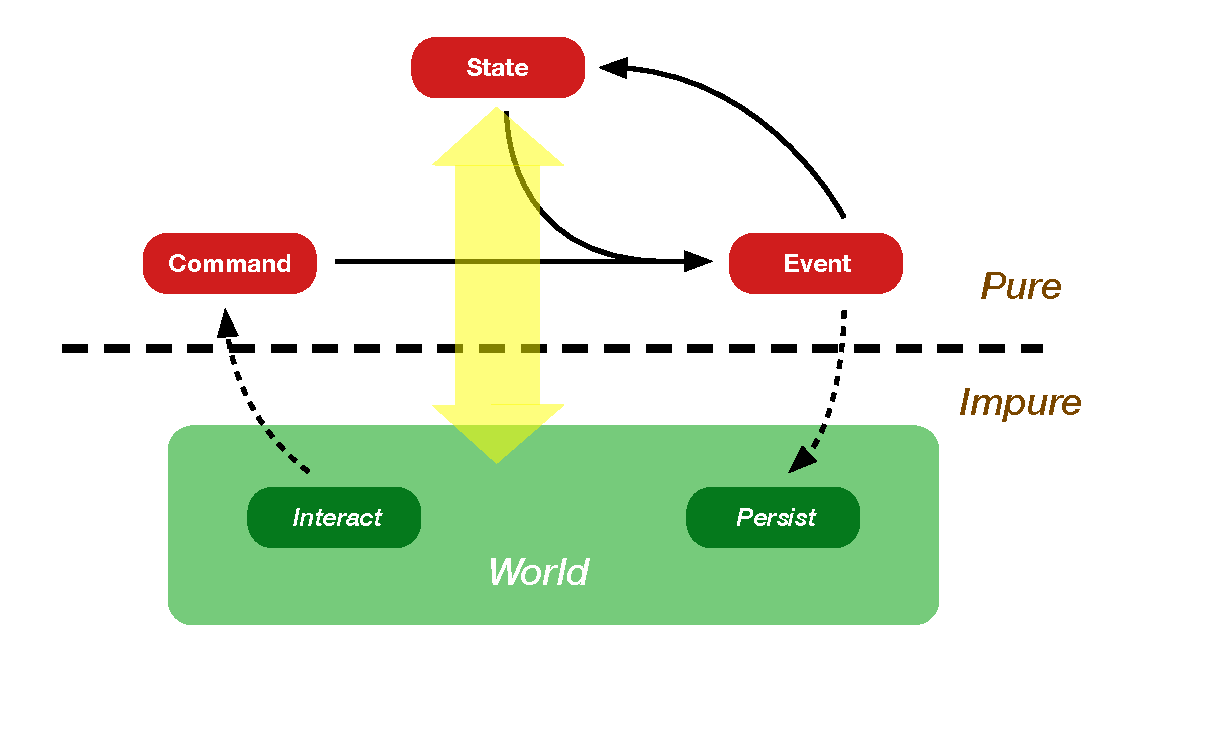
\includegraphics[width=\textwidth]{./images/event-loop.pdf}
\end{center}
\end{frame}

\begin{frame}[fragile]{Language}
  \begin{itemize}
  \item $C$ is the set of all Commands, $E$ the set of all Events, $S$ the set of states
  \item $$\delta : S \times C \times E^* \rightarrow S$$ a transition function between states $S$
  \item The language of a component $L \subseteq (C \times E^*)^*$ is a \textbf{transduction}
  \item We can simplify to $L \subseteq ((C + \epsilon) \times E)^*$
  \end{itemize}
\end{frame}

\begin{frame}[fragile]{Language}
  An \emph{Event Sourced} language is such that
  $$\forall s \in S, \exists t \in E^*, \exists c \in C^*, \delta(s_0,c \times t) = s $$
  e.g. the possible states of the system are determined by possible traces of events:
  $$S \subseteq E^*$$
\end{frame}

%%%%%%%%%%%%%%%%%%%%%%%%%%%%%%%%%%%%%%%%%%%%%%%%%%
\part{Homomorphic Event Sourcing}

\begin{frame}[fragile]{Interacting Components}
  \begin{itemize}
  \item What happens when 2 event-sourced components have to interact?
  \item Events  $E_1$ from first component must be transduced into commands $C_2$, and some events $E_2$ into $C_1$
  \item Modelling interaction as a \emph{transformation} of languages
  \end{itemize}
\end{frame}

\begin{frame}[fragile]{Base Event Loop}
\begin{center}
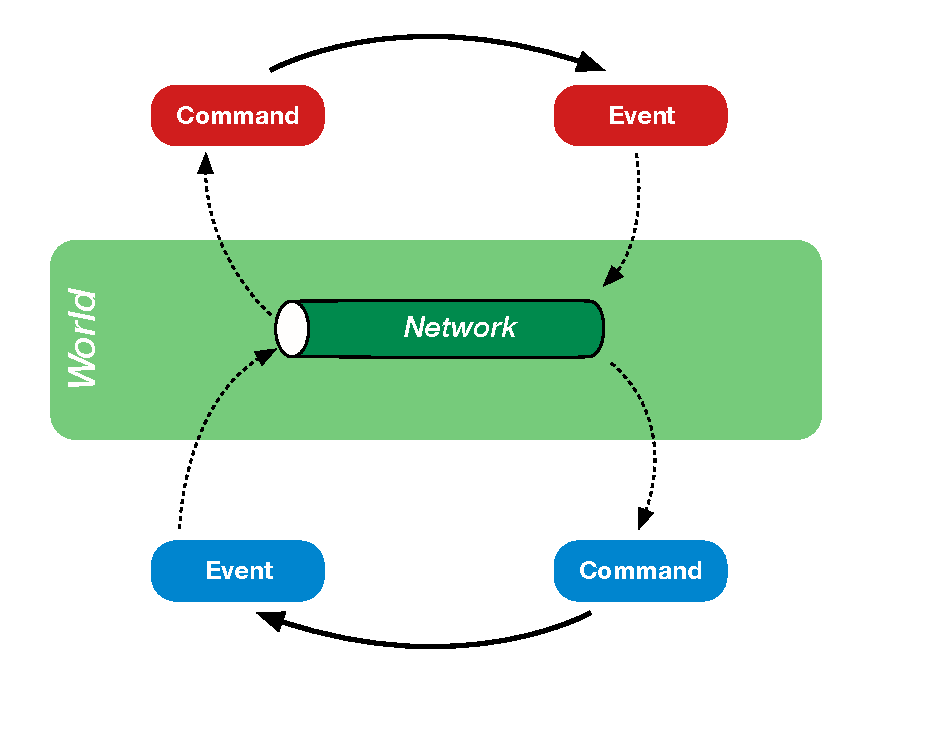
\includegraphics[height=.8\textheight]{./images/interaction-loop.pdf}
\end{center}
\end{frame}

\begin{frame}[fragile]{Homomorphism}

Let $L_1, L_2$ two languages over alphabets $\Sigma_1, \Sigma_2$, a function $\tau : L_1 \rightarrow L_2$ is a homomorphism iff

  \[
  \forall w_1, w_2 \in L_1, \tau (w_1 . w_2) = \tau (w_1) . \tau (w_2)
  \]

  In other words, a \emph{homomorphism} is a structure-preserving map between two languages. This practically means it is enough to
  define $\tau$ on $\Sigma_1$

\end{frame}

\begin{frame}[fragile]{Homomorphic Event Sourcing}
  \begin{itemize}
  \item Define mappings from UI events to backend commands: An event
    can map to nothing meaning there is not interaction with
    the backend
  \item Define mappings from backend commands to UI events: Defines how
    backend's replies are interpreted in the UI, some events might not
    be reflected in the UI (why?)
  \end{itemize}
\end{frame}

\begin{frame}[fragile]{Benefits}
  \begin{itemize}
  \item Provides a high-level understanding of how of how 2 components
    interact, e.g. a \emph{protocol}
  \item Testing:
    \begin{itemize}
    \item Mock backend to test UI only
    \item Test complete system with respect to overall model
    \item Generate tests from model against UI or backend using the
      defined language as an \emph{oracle} and \emph{generator}
    \end{itemize}
  \item Safer interactions: Define language and homomorphism in a
    single place then generate the other side
  \item Generalization to $n$ components, e.g. hexagonal architecture
  \end{itemize}
\end{frame}

\begin{frame}[fragile]{Beyond Homomorphism}
  \begin{itemize}
  \item Homomorphism do not account for \emph{current state}, e.g. what happened in the past
  \item Some events might be meaningfully interpreted only after some other events happened
  \item \emph{Homomorphism} $\longrightarrow$ \emph{Transduction}
  \end{itemize}
\end{frame}

\begin{frame}[fragile]{Transductions}
%  \begin{itemize}
%  \end{itemize}
\end{frame}

%%%%%%%%%%%%%%%%%%%%%%%%%%%%%%%%%%%%%%%%%%%%%%%%%%
\input cdct

%%%%%%%%%%%%%%%%%%%%%%%%%%%%%%%%%%%%%%%%%%%%%%%%%%
\section{Examples \& Demo}

%%%%%%%%%%%%%%%%%%%%%%%%%%%%%%%%%%%%%%%%%%%%%%%%%%
\begin{frame}{Thank you very much!}

  \url{https://github.com/}

  ~\\[1em]
  \begin{block}{Arnaud Bailly}
        \begin{description}[Twitterxx]
        \item[E-Mail]  \href{mailto:arnaud@aleryo.com}{\texttt{arnaud@aleryo.com}}
        \item[Twitter] \href{http://twitter.com/NicoleRauch}{\texttt{@dr\_c0d3}}
        \item[Web] \href{http://aleryo.com}{\texttt{http://aleryo.com}}
        \end{description}
  \end{block}
  \begin{block}{Nicole Rauch}
    \begin{description}[Twitterxx]
    \item[E-Mail]  \href{mailto:info@nicole-rauch.de}{\texttt{info@nicole-rauch.de}}
    \item[Twitter] \href{http://twitter.com/NicoleRauch}{\texttt{@NicoleRauch}}
    \item[Web] \href{http://www.nicole-rauch.de}{\texttt{http://www.nicole-rauch.de}}
    \end{description}
  \end{block}
\end{frame}
